% Project-authored fixture: illustrative measurements for a sensor calibration note.
\documentclass{article}
\usepackage{amsmath}
\usepackage{pgfplots}
\pgfplotsset{compat=1.18}

\title{Optical Sensor Calibration}
\author{Instrumentation Lab}
\date{September 2026}

\begin{document}
\maketitle

\section{Response curve}
The detector was exposed to five reference concentrations between zero and
four units. The fitted response is
\begin{equation}
S(c) = 0.5c^2 + 0.2c + 0.1.
\end{equation}
The points below are illustrative measurements. The figure compares the
measured signal with the fitted function over the calibrated range.

\begin{figure}
\centering
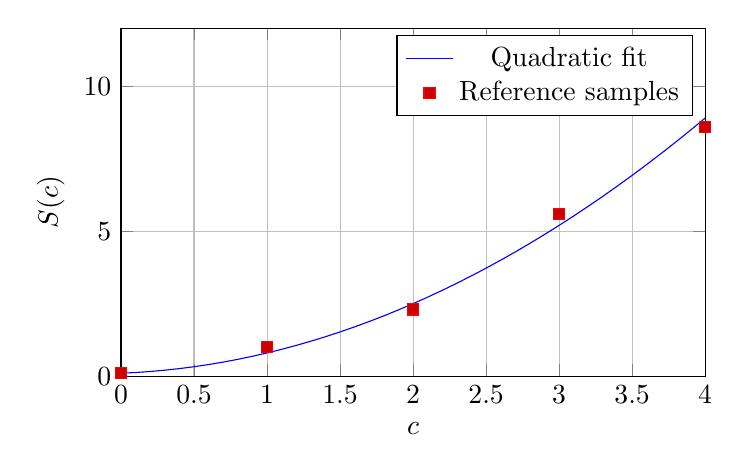
\begin{tikzpicture}
  \begin{axis}[
    xmin=0,xmax=4,ymin=0,ymax=12,
    width=9cm,height=6cm,
    xlabel={$c$},ylabel={$S(c)$},
    grid=major,domain=0:4,samples=41]
    \addplot[blue] {0.5*x^2+0.2*x+0.1};
    \addlegendentry{Quadratic fit}
    \addplot+[red,only marks] coordinates {
      (0,0.1) (1,1.0) (2,2.3) (3,5.6) (4,8.6)
    };
    \addlegendentry{Reference samples}
  \end{axis}
\end{tikzpicture}
\caption{Calibration curve and measured reference samples.}
\label{fig:calibration}
\end{figure}

The measurement at the upper end remains inside the specified signal range.
\end{document}
